\documentclass[]{article}
%\documentclass[conference]{IEEETran}
\usepackage[colorinlistoftodos]{todonotes}
%For front page purposes
\usepackage{pdfpages}
%MISC
\usepackage{framed,hyperref,url,cite}
% To handle Icelandic letters
\usepackage[utf8]{inputenc}
\usepackage[T1]{fontenc}
%\usepackage[margin=2cm]{geometry} %if we need space

%opening
\title{Like Breeder\\ \small Report in the course Procedural Content Generation in Games, Autumn 2014}
\author{Björn Þór Jónsson - \texttt{bjrr@itu.dk}\\Kasper Fryland Appeldorff - \texttt{kfap@itu.dk}}

\begin{document}
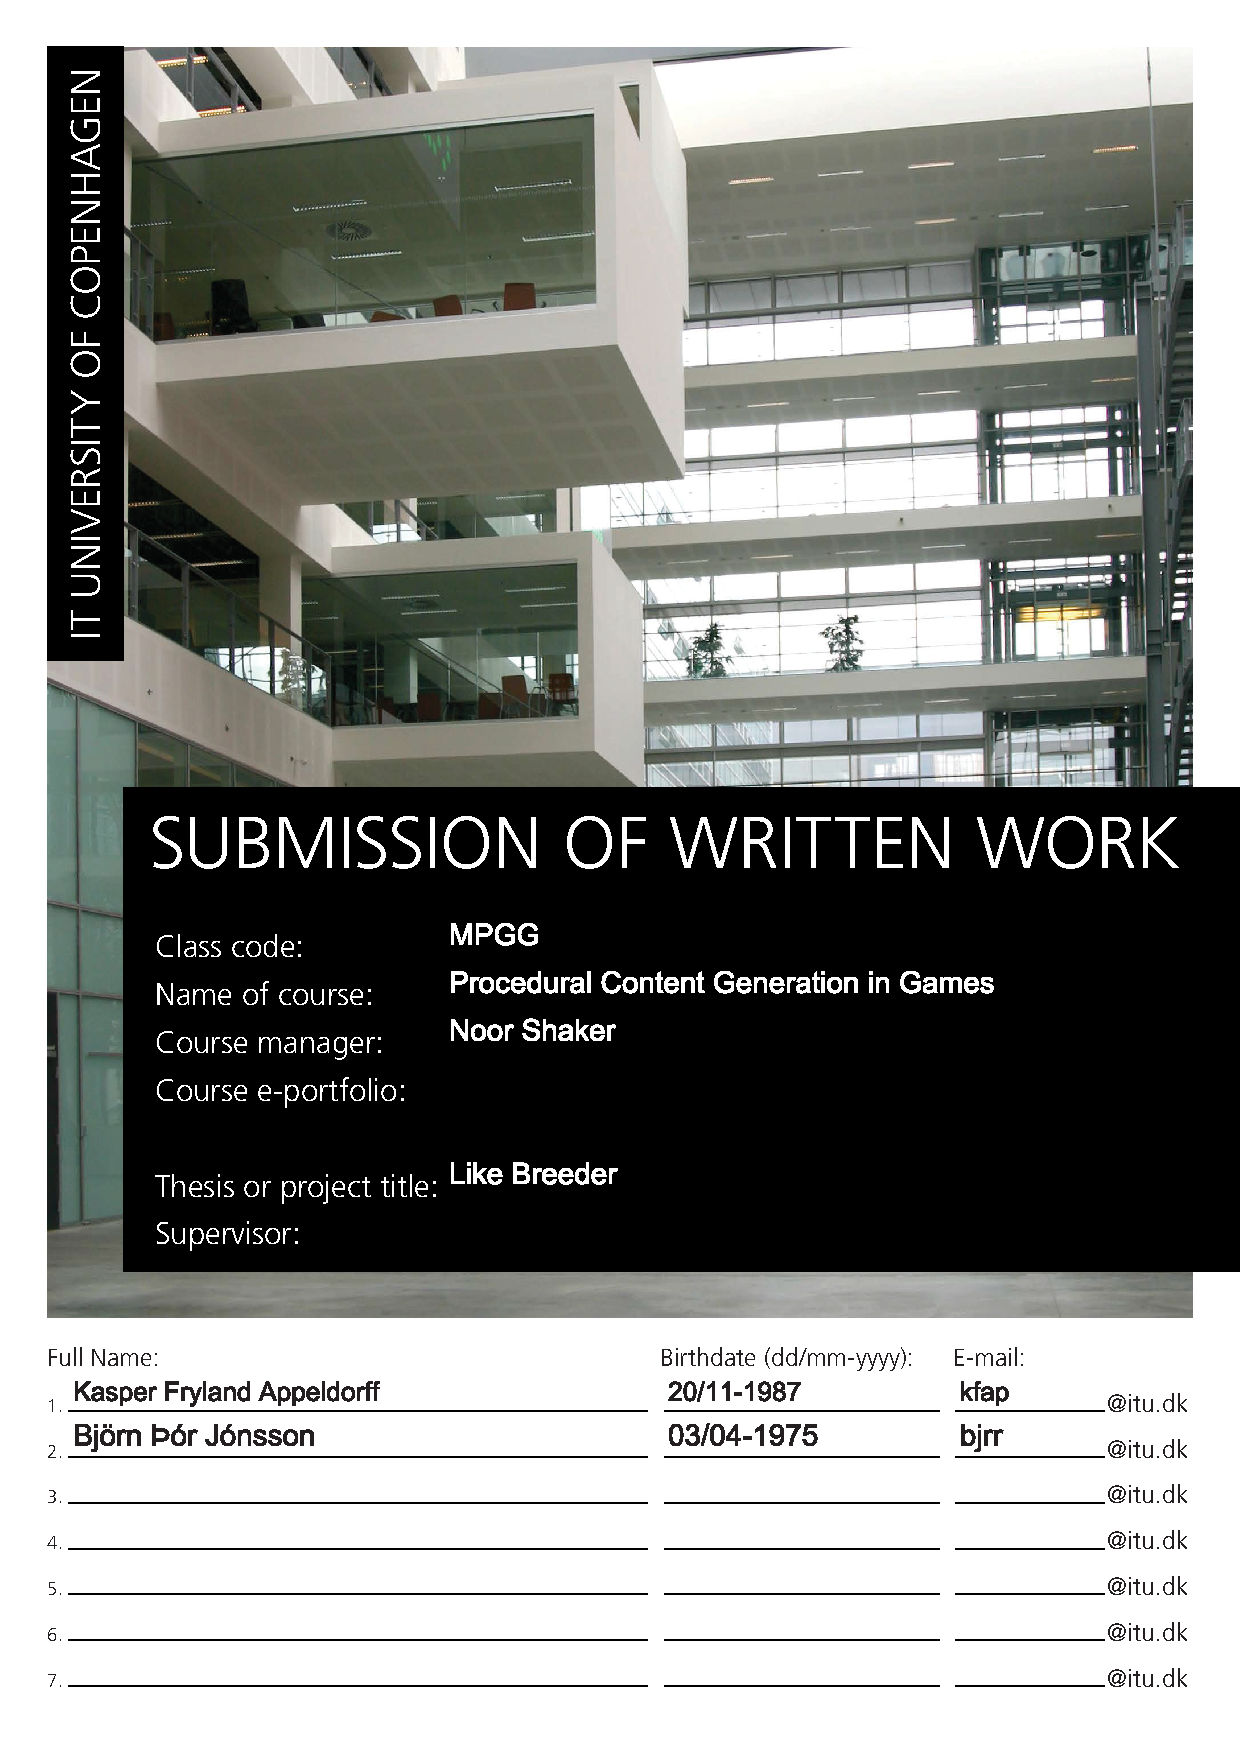
\includepdf{frontpage.pdf}
\maketitle
%\tableofcontents %Table of contents. Automagic
%\listoffigures %Also has \listoftables
\listoftodos % Requires package todonotes
\newpage
\begin{abstract}
In this report we introduce a concept of play with content provided by social media sites.  There are many conceivable scenarios for play within this concept, but our focus in this project will be on procedurally generating items that can brought as toys into those scenarios.
\end{abstract}



\section{Introduction}
\label{sec:Introduction}

\begin{center}
\textit{A mysterious new culture has been born. We are like ancient Egyptians. We communicate with pictures, we worship cats, and nobody understands us} \cite{gross2013makes}.
\end{center}


Games have become a large part of social media.  How we play can be viewed as a form of self expression \cite{sicart2014play}.  What social media items we interact with, by liking or posting them, can also be viewed as a form of self expression \cite{bargh2002can}.  Little, if anything, has been done towards creating playful activities, or games, from social media content itself.

In the wealth of social media items one may have liked or posted, are there possibly
combinations of items that better represent one's personality than others?  What if we were given the opportunity to play with the content we have liked in the past, interacting with people who like similar things, across our usual social connections, discovering new ideas and content we may like, and by the way learning more about ourselves?


\subsection{Content collection and the unconscious mind}

The Internet is full popular of social web sites \cite{LeadingSocialNetworks}, offering media of various kinds and the ability to show our appreciation in some way or another; liking, hearting, starring and so on.

Online activity involves in large part showing appreciation for the various social media items in the form of likes \cite{LM11}.  Those likes are systematically connected to form part of our online identities.  Managers of social networks have the opportunity to play with the data generated from the massive streams of likes, to profile their users, and they are likely to take that opportunity.
But what do \textit{we} use our likes for?  Do we ever revisit or reflect upon them,  or are we too busy for that, as we are constantly facing a barrage of new content?


Motivation for our ideas are the endless streams of (re)posts and likes of social media items on sites such as Tumblr\cite{1MinuteData,LM11}.  Observing that activity has lead to thoughts about whether people usually revisit the material they have interacted with, or if people continue to wade through the streams without further reflection.   Are we just continuously adding content to personal databases while never using this data to express ourselves, to define ourselves?  Are there possibly unused opportunities for self expression by reflecting on the media items connected to our online identities? \todo{merge}

If we do not revisit our previously liked items, why do we then choose to like things on social media websites?  This could prove to be a rich source ofd untapped personal content.


\subsection{Playful generation of content collections leading to self expression}

Our aim with this project is to investigate methods to engage people in reflection upon their history of online activity.  This we would like to do in a manner that would be perceived as playful, free from the tedium of manually searching ones own activity logs in a linear fashion, in hope of opening up an opportunity for self reflection that people might not have lead their thoughts to before and would welcome.

To facilitate that exploration, we have created an online environment where guests will eventually be able to connect one or more of the social media sites they use, be it Pinterest, Instagram, Tumblr, Flickr, deviantART, Spotify, SoundCloud, YouTube, etc.  To begin with, the current prototype accepts user name handles to only one of those sites:  Tumblr.  Our most basic idea is to offer the creation of cubes, where each side is decorated with a selected social media item from one's collection of likes and posts.  A future vision, which reaches outside the scope of this project, is to offer participants to bring those cubes into play with others, who bring their cubes to the table.

The prototype discussed in this report does not render the cubes visually in three dimensions, but rather presents the items, which the cubes can potentially be decorated with, on the two dimensional surface of a web page.  Though a visually stunning 3D representation may significantly support user engagement, it is the media item selection process itself that will be under consideration in this project, and the bare presentation offered here will allow evaluation of that process to be performed without distraction.

\begin{framed}
What problem are you trying to solve?Why is this important? How does this problem make some sort of game better?
\end{framed}

\section{Background}
\label{sec:Background}

While using social media content for games may be considered as novel in itself, there has been conducted research into areas that are sources of inspiration behind this project, such as those touching upon self identity and relationships between individuals based on common interests.


\subsection{Representing the self onine through avatars}

It can be said that we define ourselves by what we love.  For instance, some idea can be had about a person, by knowing what kind of music she likes, what kind of visual artwork takes her fancy, and what food she loves.  So publicly stating her likes, is a form of self expression.

%How we play, is also a form of self expression.  What kind of playful activities one seeks to participate in, and what games one likes to play, can help give an idea of what kind of person he is.  “...play is a way of engaging and expressing our being in the world.”  Play is “a way of explaining the world, others, and ourselves … who we want to be…” \cite{sicart2014play}.

Self identification is important to participants in online communities, in gaming environments, and in life in general \cite{marwick2005selling}.  “Identity plays a key role in virtual communities. In communication, which is the primary activity, knowing the identity of those with whom you communicate is essential for understanding and evaluating an interaction.  Yet in the disembodied world of the virtual community, identity is also ambiguous...” \cite{kollock2002communities}.

%An environment that combines those forms of self expression and identification - play and love of things - can provide new means of communication and discovery.  It could also foster creativity and introspection, where it allows the assembly of toys and game elements from media items of your own liking.  It is thus worthwhile to investigate the feasibility of constructing such an environment.

The importance of self identity, in online environments and games, has been given some attention in research \cite{jones1997virtual,zhao2008identity,slater2002social,kollock2002communities,marwick2005selling,vitak2008facebook}.  For instance, the importance of avatar creation, for self identification in games, has been discussed \cite{waggoner2009my,trepte2010avatar}.  The objects created from favourite media items in the process discussed in this report, the like-cubes, can be viewed as abstract avatars, portraying both a visual and a mental image of their creators \cite{trepte2010avatar}.

%Is it interesting and enjoyable to engage in online play with the social media items we have liked?  Would it be perceived as interesting to create toys from our liked media content, usable for play, games and self expression?   Would it be helpful in expressing who we really are, or who we want to be \cite{przybylski2012ideal}\todo{ref}?  Can it lead to self introspection, when given the chance to select from our likes, those that best describe our persona?  
%Is it a welcome aid in self expression, to have access to playful facilities for finding the items that best describe one's personality?
%Will it help define our real life identity?  Could it assist the formation of relationships \cite{vitak2008facebook}, when the self expression enabled by this kind of play would lead to mutual identification \cite{kimmel1966game}\todo{ref} among players?

Like Breeder is intended to aid people in profiling themselves with the media items from their personal collections.  Media sites hosting those collections may benefit from profiling users based on that data, and effort has been made in that regard, utilizing tags associated with media items \cite{guy2010social,hung2008tag}.  A significant difference presented, with the project discussed here, is that of taking steps towards placing that profiling power in the hands of the owners of the data themselves, the individual social media users.

Whereas this project is inspired by previous works on content generation with Interactive Evolutionary Computation (IEC) \cite{cardamone2011interactive,togelius2007towards,secretan2011picbreeder}, it may be viewed as novel in its use of social media items to generate content items for use in play, possibly connecting and joining their creators around common interests.\todo{couple toys to photos on cups/calendar services}

\begin{framed}
Has this been done before? How? If not, what’s the closest related research? (Both using similar approaches and other algorithms.) What’s novel with your research?
\end{framed}

\section{Game Design}
\label{sec:GameDesign}

How does this relate to games?\todo{Ref previous of no games - then make up our own}  Rating those sets of media items, with the aim of creating cubes representative of one's person, can be looked upon as a form of play, whereas games in general are one form of play.  It can be categorized as an Alea play form \cite{caillois2001man}, with a resemblance of playing a slot machine, though less random in nature while appealing to personal interests.  The cubes bred in this playful activity an can then be considered as play / game content, that can be brought by their creator into various playful activities.  With the option of 3D printing the cubes, they could become tangible toys, fit for play and games in the physical reality.

An example of a game to play, with such like-cubes, can be a quiz where two opponents are each presented with a set of three media-items-cubes and are to guess which one was created by their opponent.  Two of the cubes presented to each player are either randomly generated, selected from other user's collections, or assembled with selection based on heuristics obtained from the imported social media sites activity for each participating player, and one cube is chosen from the collection of cubes she has actually created.  Scores are given for each correct guess and players compete to become experts in each other's likes.  Such play can be viewed purely as a pastime or as a way for people to get to know each other.  Games like \textit{Guess Who?}\cite{GuessWho} can be compared to this quiz example and even inspire further elaborations on it.

Among other conceivable examples is an environment where players assemble with their cube selections, with the aim of arranging them in creative ways into strings of narratives, were short text fragments connect the cubes along interesting storylines (Figure~\ref{fig:narratives}).  Players would vote on the assembled narratives and possibly compete at receiving the most likes on their creations.  More examples of play with social media items can be conceived and a collection of possible play scenarios can be seen in \cite{GoLplay}.

\begin{figure}[h!]
	\centerline{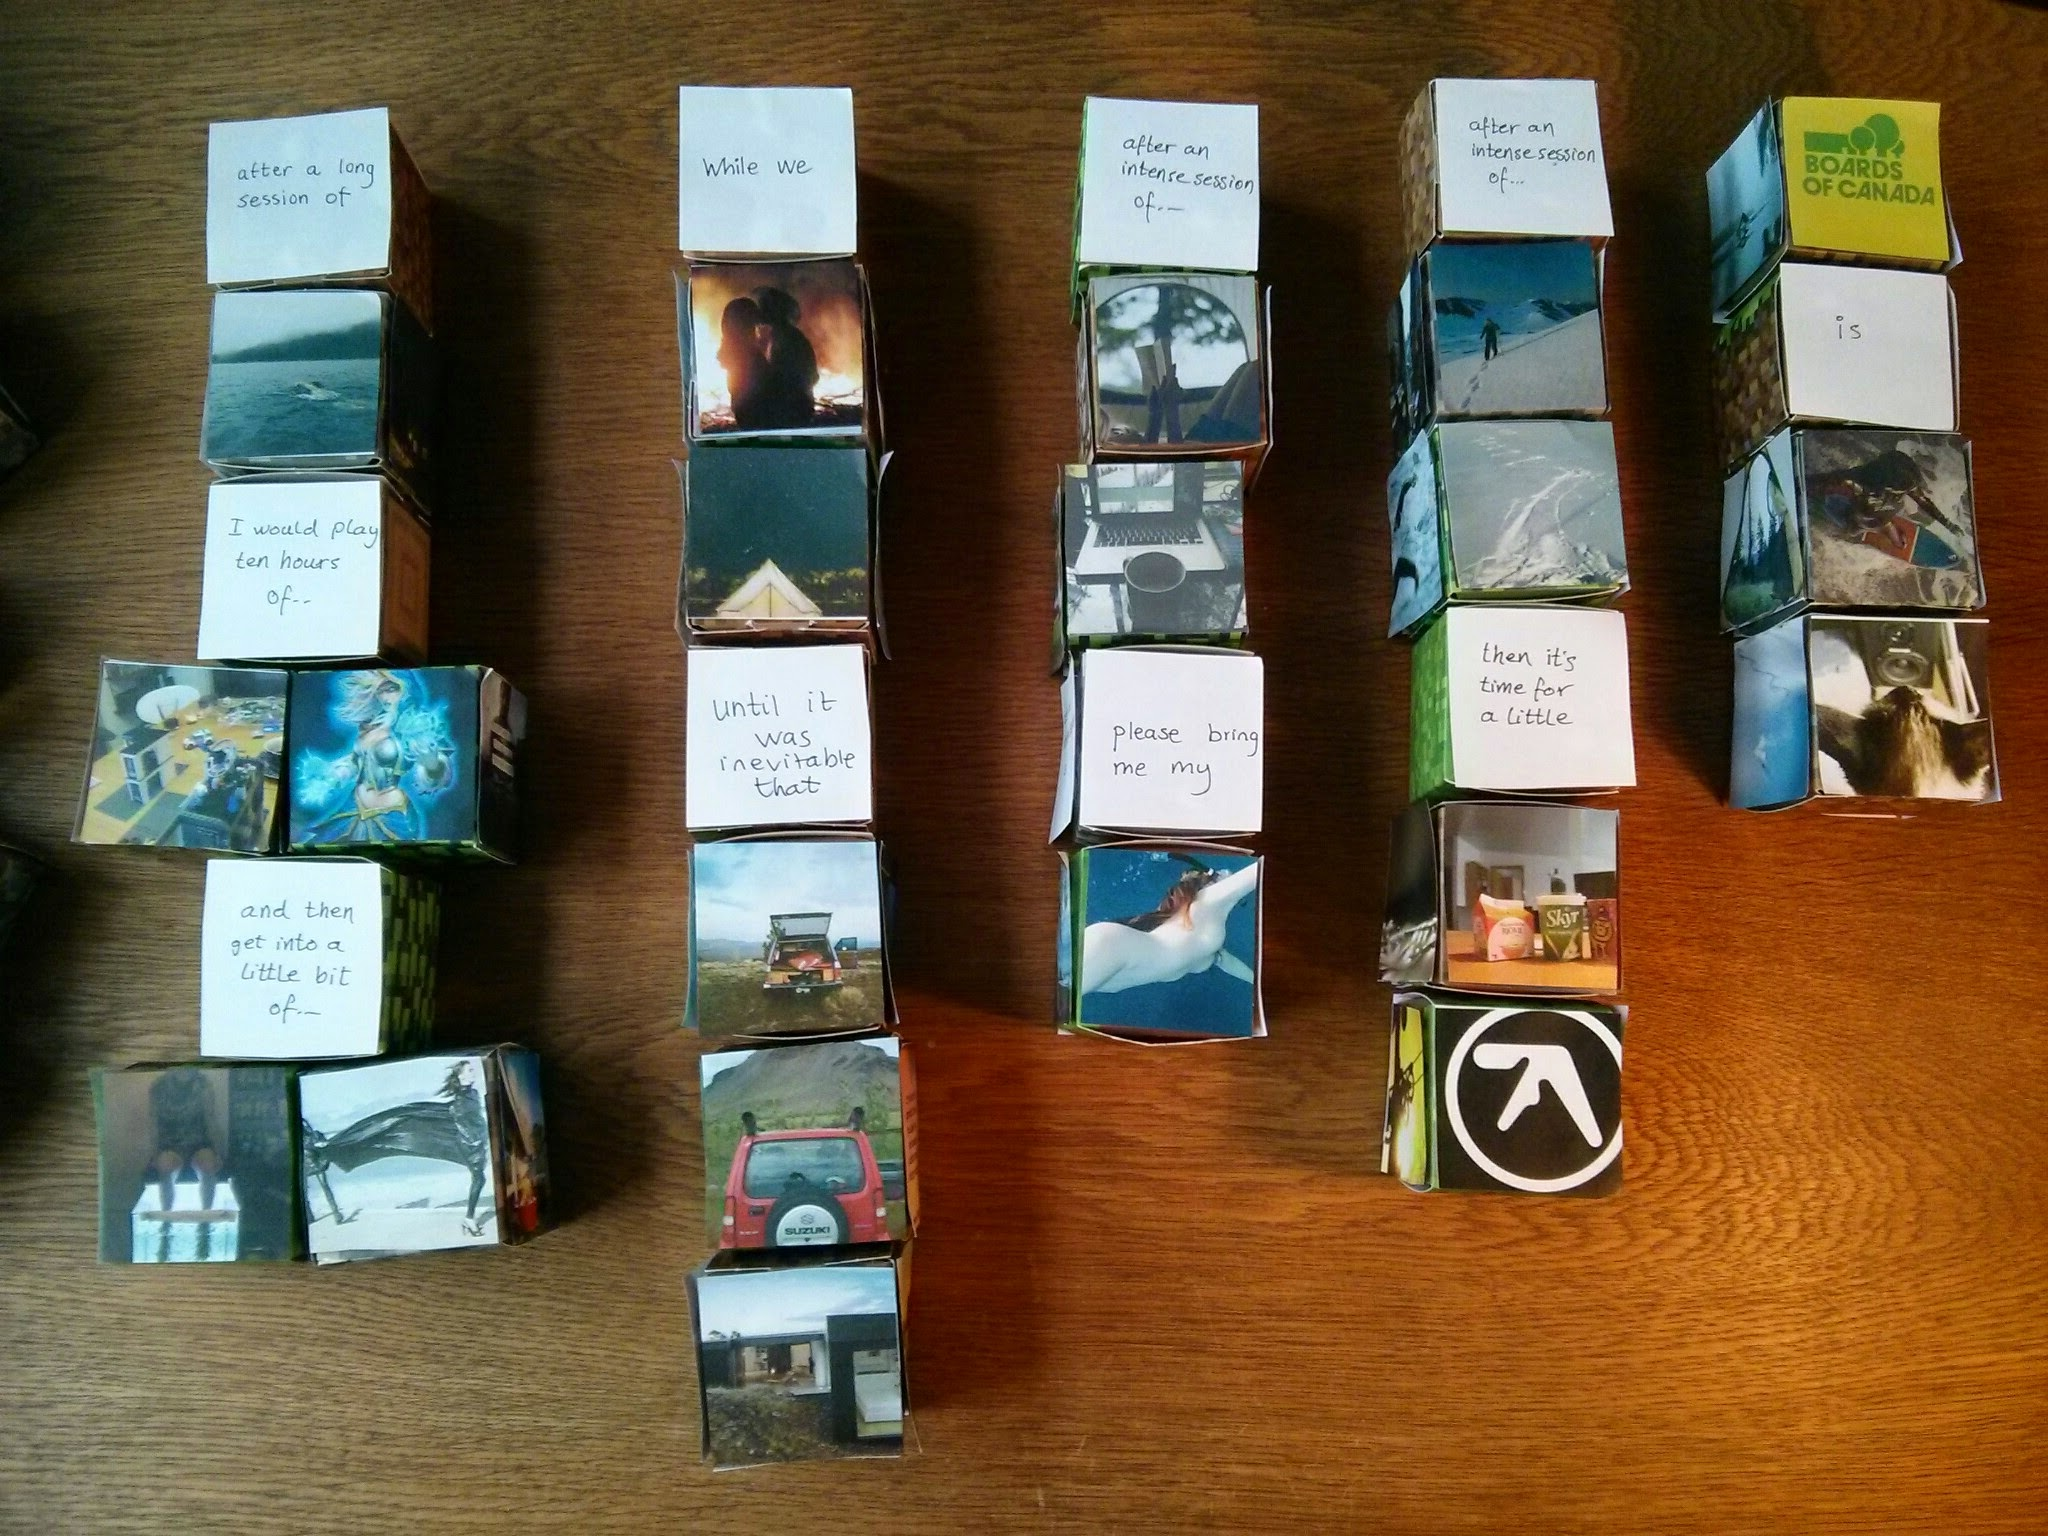
\includegraphics[width=\columnwidth]{IMG_20141029_110139.jpg}}
	\caption{Paper prototype of like-cubes at play in the creation of different narratives.}
	\label{fig:narratives}
\end{figure}

Assembling media content from ones collection of likes and posts from social media websites, by manually scanning through the items in a linear fashion, would likely be perceived as tedious work.  Aiding that activity with a variant of \textit{procedural} evolution, \textit{generating content} for social media games in a playful fashion, could increase the odds of potential players becoming engaged in that process.


\begin{framed}
What’s the design of the game you are going to use? Why do you need PCG in this game?
\end{framed}

\section{Methods}
\label{sec:Methods}

This project is inspired by the articles about IEC \cite{cardamone2011interactive,secretan2011picbreeder,togelius2007towards}.  Content presentation and user interaction is based on the discussion in that article and the related project.  Instead of composing tracks for a racing game, the aim here is to breed sets of media items that a participant finds representative of her as a person.


\subsection{Initial Genetic Algorithm design}
\label{sec:InitialAlgorithm}

Having supplied user handles for various social media networks to the like-breeding system, a participant is presented with a population created from a random selection of social media items he/she has posted or liked on the chosen networks.  In the prototype discussed in this report, access to only one network is implemented:  Tumblr.

The initial idea was to have individuals in this population composed as sets of media items, four or six in each set, and have the participant rate how well each set represents her as a person.  Then a new generation would be evolved, based on the ratings of individuals in the previous generation.  For the Genetic Algorithm, the \textit{phenotype} would be composed of the four or six media items, for decorating the sides of the “personality cube”.  
The \textit{genotype} would be an array of length four or six, of which each element is another array of tags, or if no tags accompany a media item, then the element would simply be the media item's ID / URL.
\textit{Reproduction} could be based on a crossover from the sequences of tag sets / media IDs from the parents.  
Elements in the genes of children could be copied directly from the parents or be populated with tags from new media items found in searches by the tags found in parent elements.
\begin{figure}[h!]
	\centerline{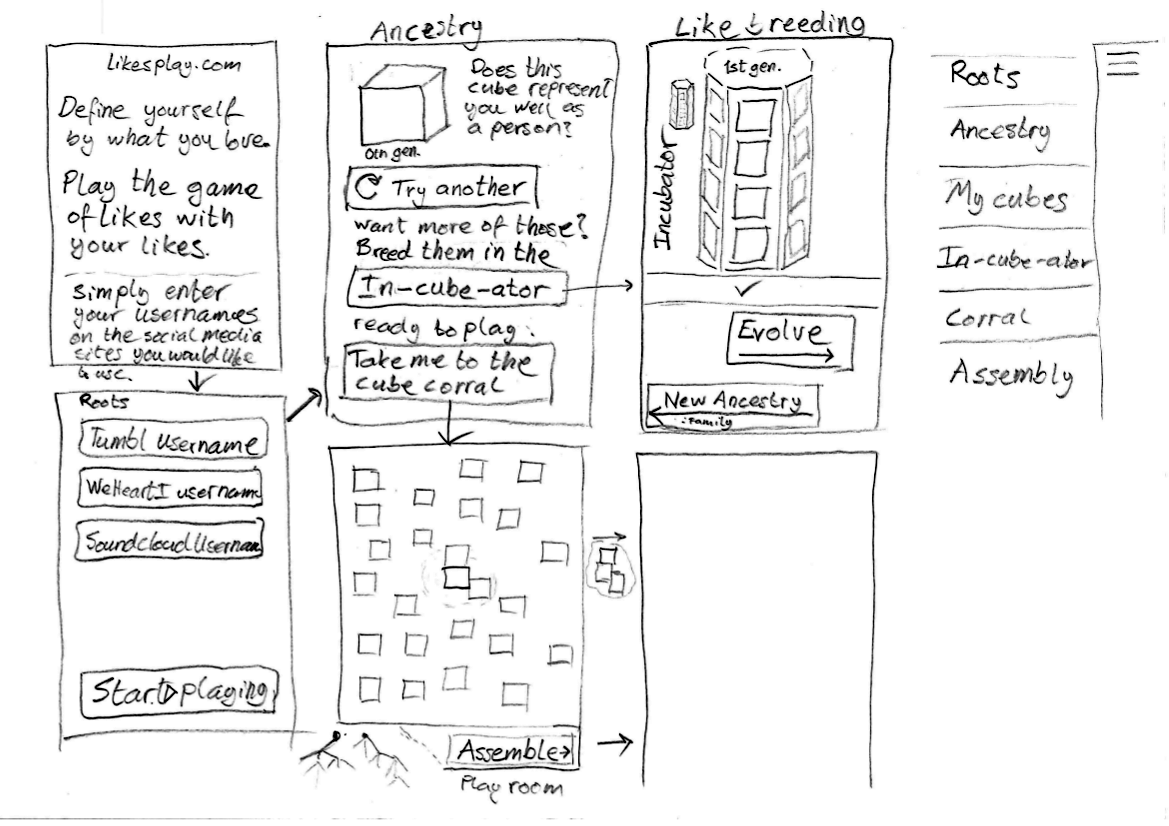
\includegraphics[width=\columnwidth]{breederUImockup.png}}
	\caption{Initial mockups of UI screens showing among other things, like-cube breeding with Interactive Evolutionary Computation, where each individual is a set of media items, and ratings are applied to each individual set.}
	\label{fig:breedingMockup}
\end{figure}


\subsection{Simplification resulting in a deviation from traditional genetic evolution}
After receiving feedback from a potential user of the breeding system, that was not involved in the project implementation, concerning the complexity of digesting multiple sets of media items at a time from one population, a decision was taken to simplify the user interface.  In an effort to lessen user fatigue, the interface was redesigned to show only one set of media items at each evolution step.  That simplified version resembles slot machines or bandits and that familiarity can be considered as an asset.  The resemblance stems especially from the change of interaction, from applying ratings to item sets to that of holding the preferred items in each given set and rolling the rest to evolve the next generation (Figure~\ref{fig:likeBreeder}).

\begin{figure}[htp]
	\centerline{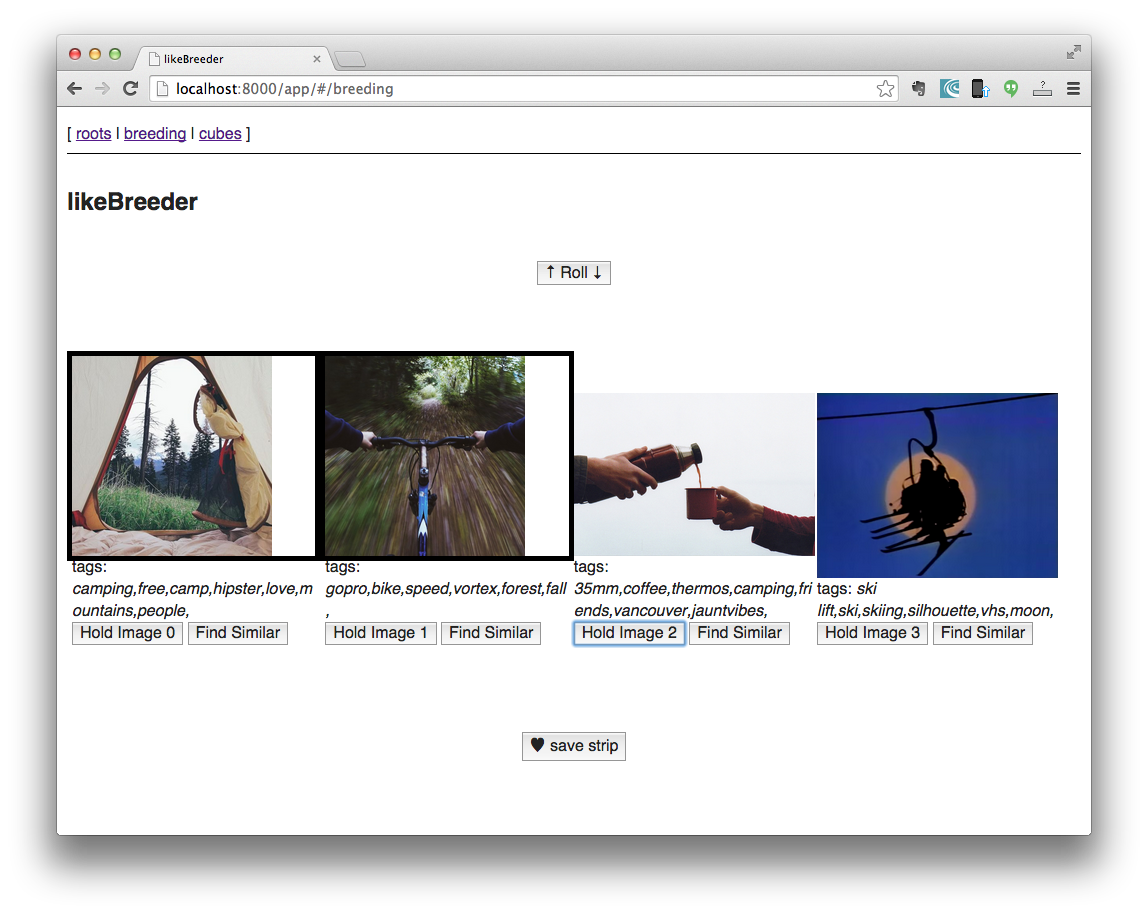
\includegraphics[width=\columnwidth]{breederPrototype2.png}}
	\caption{Screen shot of the Like Breeder prototype, with the simplified interface only showing one set of media items at a time.}
	\label{fig:likeBreeder}
\end{figure}

A result of this redesign is that our breeding algorithm has to deviate from the traditional progression of Genetic Algorithms, as there is now only one individual in the population and evaluation of fitness among individuals, selection and mating, does not apply.  As there is just the equivalent of one cube on display at a time, to lessen user fatigue, instead of many as was originally planned, there is no evolution among competing individuals.  Competition happens now among individual genes, the media items, to get a seat within the genome of that one individual.  Now there is competition among genes, rather than genotypes.


\todo{Explain how segmenting the search space would require Euclid which sucks. Unpossible to select small set of pop that adequately represents entire pop - because Euclid sucks}

\subsubsection{Measuring Similarity}
In order to find similar candidates one must first decide how to measure it. This implementations uses the Jaccard Index \cite{jaccard1912distribution}. The Jaccard Index is a similarity measure between sets. It is defined as
\begin{equation}
\label{eq:jaccard}
J(A,B) = \frac{|A \cap B|}{|A \cup B|}
\end{equation}
. In other words the Jaccard Index measures the ratio of shared elements to total elements.\\
The Jaccard Index was chosen because it was deemed fair that larger sets of tags would need to share more elements with other sets to be deemed equally similar. This is not the case with the common way of measuring similarity, Euclidean distance.\\
Euclidean distance favors small sets. This can be seen from the following example: Imagine four sets of items $S_1, S_2, S_3$ and $S_4$. $S_2$ has 2 items and one of these is found in $S_1$. $S_4$ has 100 items and 99 of those are found in $S_3$. The Euclidean distance between $S_1$ and $S_2$ is 1 and so is the distance between $S_3$ and $S_4$. Intuition says that $S_3$ should be found as more similar to $S_4$ than $S_1$ is similar to $S_2$.\\
As it turns out the Euclidean distance can expressed through the Jaccard index and the size of the union. The Euclidean distance can be simplified to $d(A,B) = \sqrt{|(A \cup B) \backslash (A \cap B)|} = \sqrt{|A \cup B| - |A \cap B|}$. From \autoref{eq:jaccard} we get that $|A \cap B| = J(A,B) \cdot |A \cup B|$ so the Euclidean distance is $d(A,B) = \sqrt{(1 - J(A,B)) \cdot |A \cup B|}$.\\
Since the union of A and B will be larger for images with many tags using the Euclidean distance will be an unfair measure.


\subsection{Suitable platforms}

Games played with social media items, such as the examples discussed in this report, fit naturally within web browser environments and are less suitable for the more traditional game engine technologies, such as those provided with Unity [ref to Unity answers], where it is more difficult to integrate online media content.  Such games could be played on mobile devices or desktop computers, running web browsers, among players geographically separated.  

To join people together, who are in the same place at the same time, in play with media items, a console gaming experience could be implemented for a web enabled device such as Chromecast \cite{ChromecastGames}, where players are joined in front of a common television screen, with game controls implemented for their mobile devices.  This would be more difficult to achieve on traditional living-room game consoles, such as the PlayStation, which do not not speak the language of the web naturally.



\begin{framed}
How does your algorithm work? Describe in as much detail as you can fit into the report. Classify your algorithm according to the taxonomy in the “Search-based Procedural Content Generation” paper. Also, how did you interface it to the game?
\end{framed}



\begin{itemize}
\item Mention that speed is fast. We might want to see if we can reach over 100k by combining blogs
\end{itemize}

\todo{mention that speed is not an issue!  cite examples...}



\section{Results}
\label{sec:Results}
No room - too bad.
\begin{framed}
Did it work? How well? Provide some figures, and a table or two. How much time does it take?
\end{framed}
\begin{itemize}		
\item It is fairly quick to reach a conclusion ie. a cube. User fatigue does not become an issue, not even close. Perhaps fiddle with set size?
	\begin{itemize}
	\item remove tags - then time (rolls + time) to complete cube
	\item Timing a few runs with test subjects might be good. We sorta know how this works and as such we are rather quick.
	\item Measure: NumRolls, Rolls giving nothing of interest, Gives up?, Subjective evaluation of topicality
	\end{itemize}
\item We should come up with some metrics - A lot of these are going to be subjective I fear.
\end{itemize}



\section{Discussion}
\label{sec:Discussion}

It could be interesting to compare our simplified version, presenting one individual and competing genes, with the initial idea, involving competition between multiple genomes and Genetic Algorithm progression in the traditional manner.  A/B testing could be employed to identify which presentation is better received by users.  It may be viewed as obvious that we have a preconceived preference for the simplified presentation, that influenced out decision to implement it in code, and so our experiments might suffer from the \textit{observer-expectancy effect}, unless they would utilize a double blind design.

\todo{...Kasper: traditional GAs employed in cube refinemenet...}
...we have considered the possibility of employing the original GA algorithm design on the set of cubes a user has already made, instead of on the whole data set (all imported media posts) as initially considered.  This could be thought of as a refinement step, where cube from ones collection are complexified, whereas the cube creation in the initial step could have tended to be more topical.  This could be done with mating, mutation and fitness evaluation as discussed in \autoref{sec:InitialAlgorithm}  ...as discussed in section....

The Like Breeder has an obvious potential to adapt content to individual preferences, as that is the essence of the content generating interaction implemented in the project discussed in this report.  Future iterations on the prototype may offer the incorporation of more social media sites, expanding its reach into the existing personal databases behind ones expressed tastes and interests, empowering their owner to portray their identity with the rich media contained within them.  This could result in a move towards singularity between the self conscious identity and that stored and presented in social media.

\begin{framed}
What are the strengths and shortcomings of your method? How well would it generalize to other game genres? How controllable is it, and what is the potential for using to adapt content to individual preferences? How would you develop it further, if you had time?
\end{framed}
\begin{itemize}
\item Shortcomings and strengths:
	\begin{itemize}
	\item Shortcoming: Not very advanced - We essentially use a matrix of indices
	\item Shortcoming: Pretty close to deterministic - Removes a bit of ``cool factor'' in my opinion. More of a subjective shortcoming but there it is. Not sure how we could ``fix'' this.
	\item Advantage: Does not ignore anything. When you get something back everything has been considered. No estimations etc.
	\item Advantage: Speed. Even with a large quantity of content updates are seemingly instant. Perhaps use this as an argument for not trying to reduce search space?
	\end{itemize}
\item  It seems very controllable to me. It depends on the amount of ``crap tags'' you put on your things but you can say that about any dataset - low quality data $\Rightarrow$ low quality results. 
\item Potential for individual preferences? Perhaps a dial or something for image set size. Other than that it is pretty customizable. You don't even need to have content you like - as long as you know where you can find it.
\item I would still look into some way of ``surprising'' the user. Instead of random/similar maybe finding dissimilar instead of random? Work under the assumption that not held / not similar means something different than what is there.

\item Establishing relationships between tags or other associated descriptive words, could be helpful. Semantic relationships, rather than the Jaccardian distances currently employed.  How can they be found?  Could something like ConceptNet help in that regard?  http://conceptnet5.media.mit.edu  

\end{itemize}
\subsection{Who did what}
\begin{itemize}
\item Björn: API communication, Initial setup
\item Kasper: Similarity computation, Layout 
\item Both: Algorithm, Report
\end{itemize}

\bibliographystyle{unsrt}
\bibliography{references}
\end{document}
